\documentclass[a4paper,12pt,titlepage]{article}
\usepackage[pdftex]{graphicx}
\usepackage[headheight=15pt]{geometry}

\usepackage{fancyhdr}
\pagestyle{fancy}
\lhead{Exercises}
\chead{}
\rhead{Power of Topology}

\usepackage[english]{babel}									
\usepackage[utf8]{inputenc}	

\usepackage{array}
\usepackage{colortbl}

\usepackage{upquote}
\usepackage{listings}
\renewcommand{\lstlistlistingname}{List of Listings}
\lstset{language=SQL}
\lstset{frame=single}
\lstset{keywordstyle=\color{blue}}
\lstset{basicstyle=\ttfamily,columns=flexible}
\lstset{breaklines=true}
\lstset{numbers=left, numberstyle=\tiny, stepnumber=1, numbersep=5pt}

\usepackage[section]{placeins}
\usepackage{float}

%PDF hyperlinks
\usepackage[colorlinks=true,linkcolor=orange,citecolor=blue,bookmarksopen=true,bookmarksnumbered=true,pdfstartpage=1]{hyperref}
\hypersetup{
	pdftitle={Power of Topology},
	pdfauthor={Michael Wagner},
	pdfsubject={Topology, pgRouting, PostgreSQL, PostGIS},
	pdfkeywords={Topology, pgRouting, PostgreSQL, PostGIS, GIS, QGIS}
}

\usepackage[nonumberlist,nopostdot]{glossaries}
% Set width of the abbreviation column
\setglossarystyle{alttree}
\glssetwidest{SWIO-RAFI-XX}
%
\makeglossaries
\loadglsentries{abbr}
\setacronymstyle{long-short}

\usepackage{color}
\definecolor{orange}{rgb}{1,.5,0}


\title{Exercises: Power of Topology}
\author{Michael Wagner (mwagner@allspatial.info)}


\date{July 15, 2016}     													

\clubpenalty=4500																
\widowpenalty=10000								
\linespread{1.3}

%%-------------------------Document begins--------------------------------------------
\begin{document}             											% End of preamble and beginning of text.
\maketitle                   											% Produces the title.

% Inhalts-, Abbildungs- und Tabellenverzeichnis
\tableofcontents
\listoffigures
\lstlistoflistings
%\listoftables
\newpage
\printglossary[type=\acronymtype,title={List of Abbreviations}]
\newpage

\section{Introduction}

In this exercise you will do various analyses based on topology:

\begin{itemize}
	\item Shortest path analysis with the QGIS Road Graph plugin
	\item Shortest path analysis using pgRouting, a routing extension for PostgreSQL/PostGIS
	\item Generating a map of service areas that will show in what time the \gls{sfrsa} can reach what areas
\end{itemize}


\section{Data preparation}

For the road network you will make use of the \textit{road} table from your database \textit{my\_first\_geodb} that you created yesterday. This table needs a little bit of fixing and cleaning before we will start with any analysis. In \textit{pgAdmin} connect to database \textit{my\_first\_geodb} and open a new SQL query dialog. We will first delete a number of columns that are not needed:

\begin{lstlisting}[caption={Deleting columns}]
ALTER TABLE vector_data.road DROP COLUMN numberofla;
ALTER TABLE vector_data.road DROP COLUMN pavementty;
ALTER TABLE vector_data.road DROP COLUMN island;
ALTER TABLE vector_data.road DROP COLUMN cost_fp;
ALTER TABLE vector_data.road DROP COLUMN reverse_01;
\end{lstlisting}

Then rename the column \textit{reverse\_co} to \textit{reverse\_cost}. Because of the Shapefile limitation of 10 characters for field names the original field name was cut off.

\begin{lstlisting}[caption={Renaming a column}]
ALTER TABLE vector_data.road RENAME COLUMN reverse_co TO reverse_cost; 
\end{lstlisting}

During the Shapefile import all fields of data type integer were converted to float types. We will fix that and change their data type back to integer:

\begin{lstlisting}[caption={Changing a column's data type}]
ALTER TABLE vector_data.road ALTER direction TYPE int4;
ALTER TABLE vector_data.road ALTER category TYPE int4;
ALTER TABLE vector_data.road ALTER speedlimit TYPE int4;
ALTER TABLE vector_data.road ALTER condition TYPE int4;
ALTER TABLE vector_data.road ALTER source TYPE int4;
ALTER TABLE vector_data.road ALTER target TYPE int4;
\end{lstlisting}

Finally we will empty the table to load a topological clean dataset afterwards:

\begin{lstlisting}[caption={Deleting data from a table}]
DELETE FROM vector_data.road; 
\end{lstlisting}

From within the SQL query dialog load the \textit{road\_data\_cleaned.sql} script (folder \textit{Data/RoadData}) and run it. This will populate the currently empty \textit{road} table with topologically clean road data for Mahe.

\section{Shortest path analysis with the QGIS Road Graph plugin}

Launch QGIS and load the \textit{road} layer from the \textit{my\_first\_geodb} database. Load the aerial photo of Mahe from the \textit{Data/AerialPhoto} folder. Open the \textit{Manage and Install Plugins} dialog from the \textit{Plugins} menu. Search for \textit{Road Graph} and activate the plugin. A new dock widget titled \textit{Shortest path} should appear below the table of contents (Figure \ref{fig:road_graph_dwidget}).

\begin{figure}[htb]
	\centering
	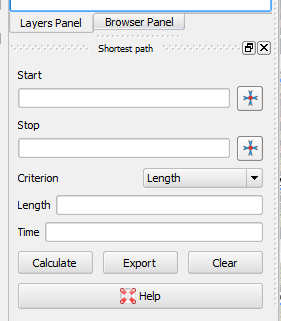
\includegraphics[width=5cm]{Images/road_graph_dwidget.png}
	\caption{Widget for shortest path analysis}\label{fig:road_graph_dwidget}
\end{figure}

From menu \textit{Vector:Road graph} open the \textit{Settings} dialog and set the parameters as shown in Figure \ref{fig:road_graph_settings1}.

\begin{figure}[htb]
	\centering
	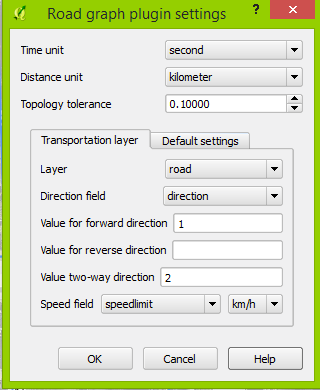
\includegraphics[width=5cm]{Images/road_graph_settings1.png}
	\caption{Road Graph plugin configuration}\label{fig:road_graph_settings1}
\end{figure}

The topology tolerance is set to 0.1 (10cm). Any two line ends within 10cm distance are considered to be connected to the same node. For a road network five to ten centimetres should be a reasonable tolerance value. The \textit{road} table has a column with information about the direction (\textit{direction}) and the speed limit (\textit{speedlimit}). A value of 1 for direction means one-way road, a value of 2 stands for both directions. Zoom the map to somewhere near the cathedral in Victoria. In the \textit{Shortest path} widget click the cross-hair button next to the \textit{Start} field and click near the junction labelled with \textit{F} in Figure \ref{fig:define_path}. Click the cross-hair button next to the \textit{Stop} field and click near the junction labelled with \textit{T} in Figure \ref{fig:define_path}. Finally click the \textit{Calculate} button. The shortest path will be shown in the map and the time and distance calculated.

\begin{figure}[htb]
	\centering
	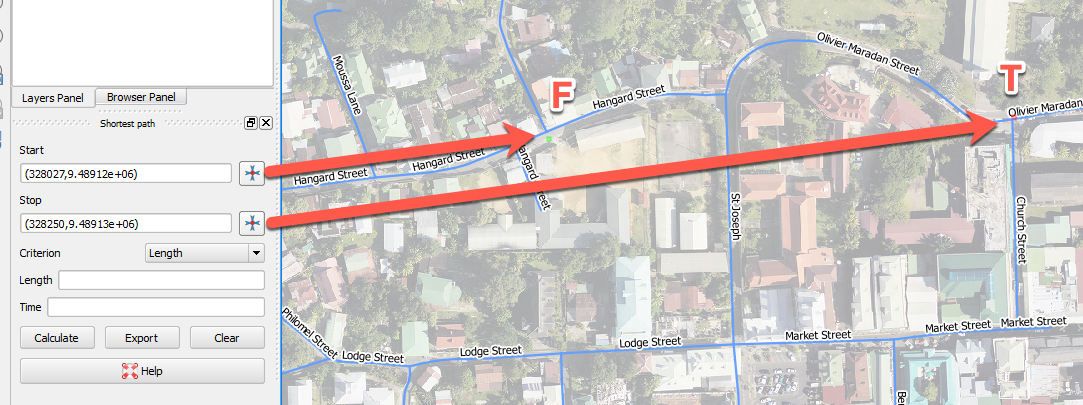
\includegraphics[width=12cm]{Images/define_path.png}
	\caption{Define start and destination for the shortest path analysis}\label{fig:define_path}
\end{figure}

Now repeat the analysis but swap \textit{Start} and \textit{Stop} point before. This time you should get a different result. This is because some of the road segments are one-way only and thus, the shortest path is calculated accordingly (Figure \ref{fig:path1}).

\begin{figure}[htb]
	\centering
	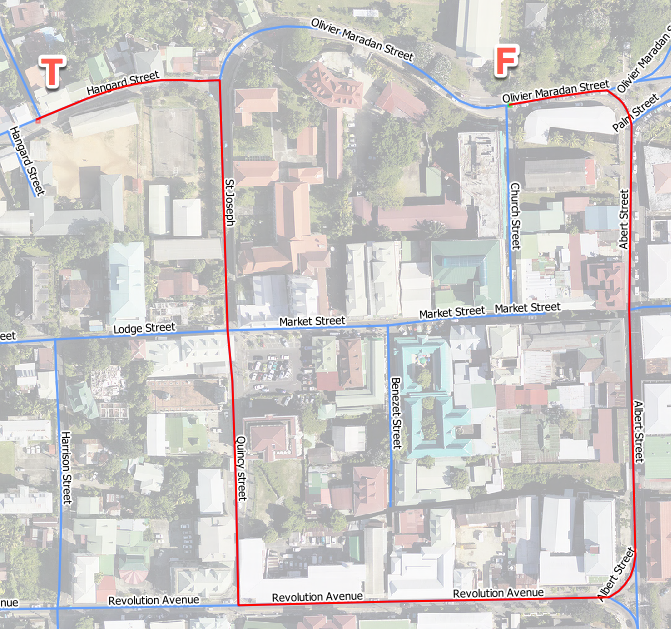
\includegraphics[width=7cm]{Images/path1.png}
	\caption{Analysis result}\label{fig:path1}
\end{figure}

In the \textit{Shortest path} widget change the \textit{Criterion} field from \textit{Length} to \textit{Time} and click the \textit{Calculate} button again. The result will be the same as before since with the currently defined speed limits no other path would save more time. Now edit the \textit{road} layer and reduce the speed limit on \textit{Quincy Street} from 50 to 5 km/h. Repeat the analysis by clicking the \textit{Calculate} button again. You should get a different result this time.

Sometimes it is useful to visualise the default direction of the road segments. You can do that by adding a \textit{Marker Line} to your simple line currently used for the \textit{road} layer style. The result might look like in Figure \ref{fig:visualise_direction}.

\begin{figure}[htb]
	\centering
	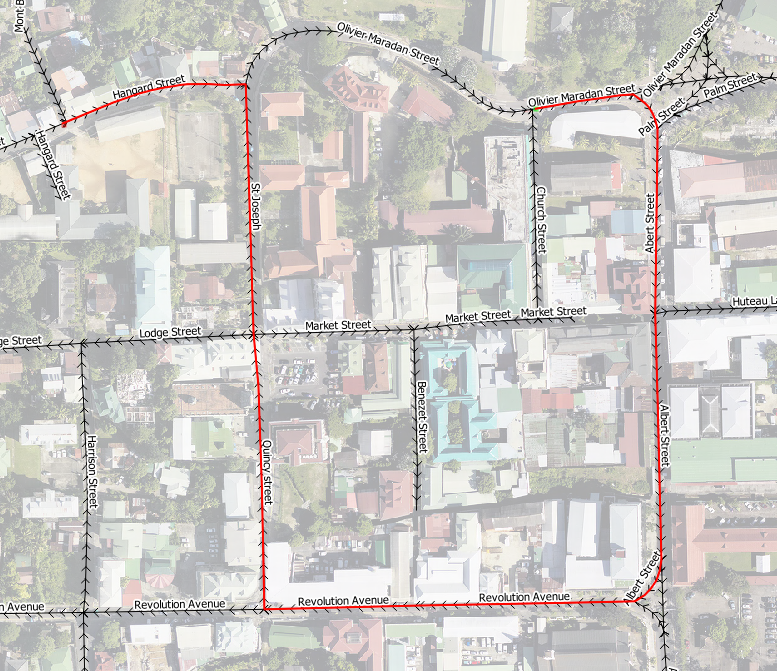
\includegraphics[width=7cm]{Images/visualise_direction.png}
	\caption{Visualise road directions}\label{fig:visualise_direction}
\end{figure}

\section{Shortest path analysis with pgRouting}

\textit{pgRouting} is an extension for PostgreSQL/PostGIS to add routing functionality on database level. Thus, the routing engine is basically the database. The advantage is that all calculation is done on the server (which would often have more computing power than a laptop or desktop). Different client applications (e.g. QGIS or a web or mobile application) then just need to visualise the results. pgRouting requires PostGIS to be installed and loaded in the database to use pgRouting with. Your database \textit{my\_first\_geodb} has the PostGIS extension already loaded. What is left is to load is the pgRouting extension itself. Loading an extension can only be done by a database superuser. Using pgAdmin connect to database \textit{my\_first\_geodb} as user \textit{postgres} and open an SQL query dialog. Run the following statement to load the pgRouting extension:

\begin{lstlisting}[caption={Loading pgRouting extension}]
CREATE EXTENSION pgrouting; 
\end{lstlisting}

Open another SQL query dialog for \textit{my\_first\_geodb}, this time as user \textit{geodb\_admin}. There is some more preparation we need to do before we can run a pgRouting analysis. We have to set the \textit{source} and \textit{target} columns to NULL because we want to build new topology in a moment.

\begin{lstlisting}[caption={Setting columns to NULL}]
UPDATE vector_data.road SET source = NULL, target = NULL;
\end{lstlisting}

Next, we will create proper topology for our road data. pgRouting provides a helper function to do that. This function will first create a new table named \textit{road\_vertices\_pgr} and populate it with the nodes. pgRouting will then populate the \textit{source} and \textit{target} columns of our \textit{road} table with the IDs of the relating nodes. The function is called like so:

\begin{lstlisting}[caption={Building topology for the road data}]
SELECT pgr_createTopology('vector_data.road', 0.1, 'geometry', 'gid');
\end{lstlisting}

The function expects the follows parameters:

\begin{itemize}
	\item Schema and table name of the edge table
	\item Tolerance (0.1m)
	\item Name of the geometry column
	\item Name of the primary key column
\end{itemize}

Now we will populate the cost columns of the \textit{road} table. The costs are crucial because based on the costs pgRouting will calculate the shortest path. We will use length and speed limit of the road segments to calculate the costs as time in minutes needed to travel a segment. We set the \textit{reverse\_cost} to same value as \textit{cost} and set \textit{reverse\_cost} to -1 for all one-way roads.

\begin{lstlisting}[caption={Calculating cost values}]
UPDATE vector_data.road SET cost = ((ST_Length(geometry)/1000)/speedlimit)*60;
UPDATE vector_data.road SET reverse_cost = cost;
UPDATE vector_data.road SET reverse_cost = -1 WHERE direction = 1;
\end{lstlisting}

Next, grant a SELECT privilege on the node table:

\begin{lstlisting}[caption={Granting SELECT on node table}]
GRANT SELECT ON vector_data.road_vertices_pgr TO gis_update, gis_view;
\end{lstlisting}

Load the node table (\textit{road\_vertices\_pgr}) in QGIS and label it with the node IDs. Write down the node IDs of two nodes that you want to find the shortest path between. Run the following query to perform the shortest path analysis using the \textit{Bidirectional Dijkstra-Algorithm} and replace 281 and 500 with the IDs of the nodes that you chose as start and end point of your analysis.

\begin{lstlisting}[caption={Shortest path analysis with bddijkstra}]
SELECT * FROM pgr_bddijkstra('SELECT gid::int4 AS id, source::int4, target::int4, cost::float8, reverse_cost::float8 FROM vector_data.road', 281, 500, true, true);
\end{lstlisting}

Figure \ref{fig:routing_result} shows an example result of the shortest path analysis using the \textit{Bidirectional Dijkstra Algorithm}. Column \textit{id1} contains the IDs of the nodes while column \textit{id2} contains the IDs of the edges. The \textit{cost} column contains the cost (in minutes) to travel the particular edge.

\begin{figure}[htb]
	\centering
	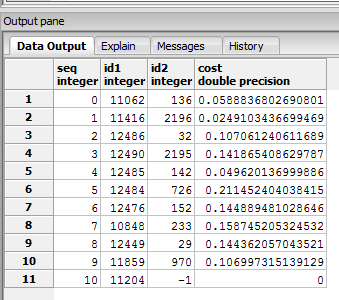
\includegraphics[width=7cm]{Images/routing_result.png}
	\caption{Example result of shortest path analysis (bddijkstra)}\label{fig:routing_result}
\end{figure}

To visualise the shortest path in QGIS we can create a spatial view. As user \textit{user\_name} open an SQL query dialog for database \textit{my\_first\_geodb} in pgAdmin. Run the query as follows to create the spatial view:

\begin{lstlisting}[caption={Create a spatial view to visualise the analysis results}]
CREATE OR REPLACE VIEW shortest_path AS
SELECT * FROM vector_data.road WHERE gid IN
(SELECT id2 FROM pgr_bddijkstra('SELECT gid::int4 AS id, source::int4, target::int4, cost::float8, reverse_cost::float8 FROM vector_data.road', 281, 500, true, true));
\end{lstlisting}

Load this view into QGIS and select the \textit{gid} as the Feature ID column. Creating a spatial view for each query result is not too convenient. It would be much better to have a tool available similar to the Road Graph plugin. Fortunately there is such tool. From the \textit{Manage and Install Plugins} dialog install the \textit{pgRoutingLayer} plugin. This plugin supports visualising the results of most of the algorithms pgRouting provides. In the \textit{pgRouting Layer} widget do the settings as shown in Figure \ref{fig:pgrouting_plugin}.

\begin{figure}[htb]
	\centering
	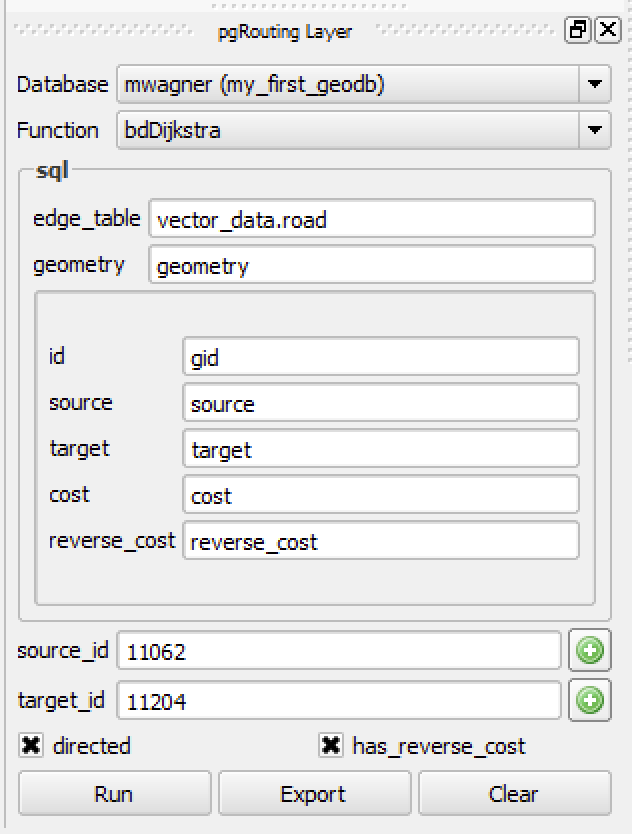
\includegraphics[width=7cm]{Images/pgrouting_plugin.png}
	\caption{Settings for \textit{pgRouting Layer} plugin}\label{fig:pgrouting_plugin}
\end{figure}

Set the source and target point in the map using the button next to the \textit{source\_id} and \textit{target\_id} field and click \textit{Run}. pgRouting will calculate the shortest path and the plugin will visualise it in the map.

\section{Identifying service areas}

We want to find out in what time the \gls{sfrsa} teams at the two fire stations on Mahe can reach what area. This type of analysis can help them improving their response times for example. Load the \textit{fire\_station} Shapefile from the \textit{Data/Shapefiles} folder. Visually identify the node that is nearest to each station and write down the ID of these nodes, e.g. the nearest node in Figure \ref{fig:nearest_node} would be 12276 (node in grey, station in green). 

\begin{figure}[htb]
	\centering
	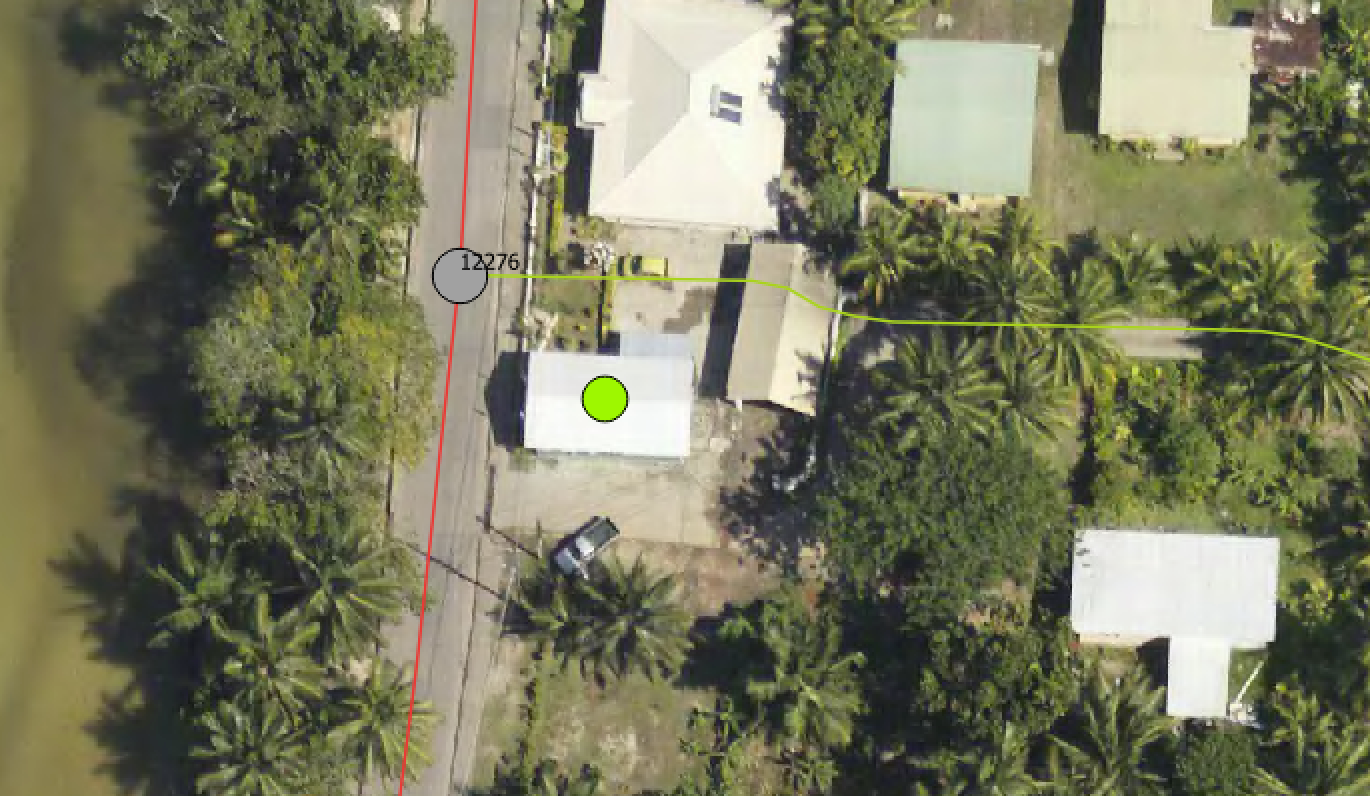
\includegraphics[width=10cm]{Images/nearest_node.png}
	\caption{Identifying nearest node to station}\label{fig:nearest_node}
\end{figure}

Run the following SQL statement to calculate the costs (i.e. the time) for travelling from these two nodes to every other node in the road network and create a table with the results. Replace the IDs 11127 and 11292 with the IDs of the nodes that you identified as closest to the fire stations.

\begin{lstlisting}[caption={Calculating travelling costs}]
CREATE TABLE combined_driving_times AS
SELECT
    id,
    the_geom,
    (select sum(cost) FROM
    (
    SELECT * FROM pgr_bddijkstra('SELECT gid::int4 as id, source::int4, target::int4, cost::float8, reverse_cost::float8 FROM vector_data.road', 11127, id::int4, TRUE, TRUE)) as foo) AS cost
    FROM vector_data.road_vertices_pgr
UNION
SELECT
    id,
    the_geom,
    (select sum(cost) FROM
    (
    SELECT * FROM pgr_bddijkstra('SELECT gid::int4 as id, source::int4, target::int4, cost::float8, reverse_cost::float8 FROM vector_data.road', 11292, id::int4, TRUE, TRUE)) as foo) AS cost
    FROM vector_data.road_vertices_pgr;
\end{lstlisting}
 
The new table will have two travelling cost entries for each node but we are only interested in the one that is lowest. Run the statement as follows to create a new table with only the minimum costs. 

\begin{lstlisting}[caption={Extracting minimum travelling costs}]
CREATE table min_driving_times AS
SELECT id, the_geom, min(cost) AS cost
FROM combined_driving_times
GROUP BY id, the_geom;
\end{lstlisting}

Load the \textit{min\_driving\_times} table into QGIS. We will now create a cost surface by interpolating the costs from the \textit{min\_driving\_times} table. In this cost surface each cell represents the travelling time to reach that cell. Select the \textit{Interpolation} tool from the \textit{Raster} menu. Apply the settings shown in Figure \ref{fig:cost_surface_settings} and click \textit{Ok}. Generating the cost surface might take a few seconds.

\begin{figure}[htb]
	\centering
	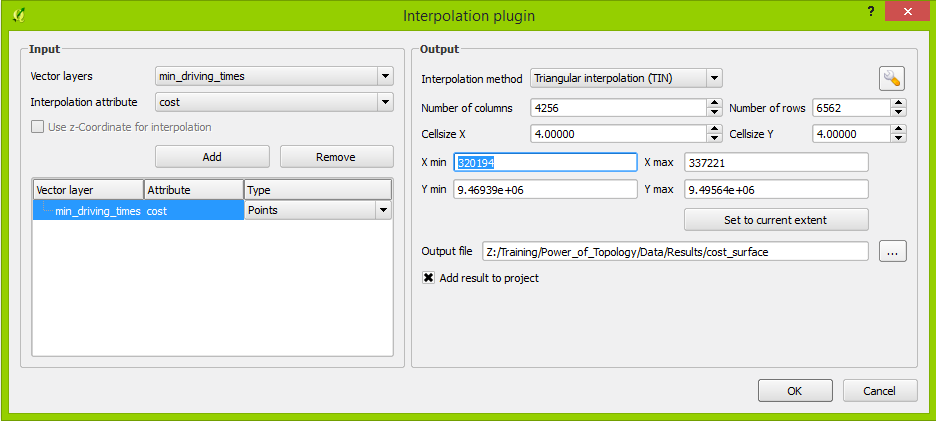
\includegraphics[width=12cm]{Images/cost_surface_settings.png}
	\caption{Settings to generate the cost surface}\label{fig:cost_surface_settings}
\end{figure}
 
We can now generate isochrones (lines connecting points of the same time interval) from the cost surface. Select the \textit{Contour} tool from the \textit{Raster:Extraction} menu and apply the setting shown in Figure \ref{fig:contour_settings}.

\begin{figure}[htb]
	\centering
	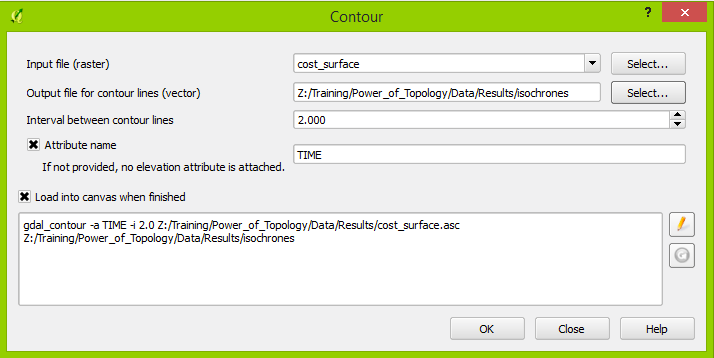
\includegraphics[width=12cm]{Images/contour_settings.png}
	\caption{Settings to generate the isochrones}\label{fig:contour_settings}
\end{figure}

Finally we will clip the \textit{cost\_surface} and \textit{isochrones} layers to the outline of Mahe. Load the \textit{mahe\_island} Shapefile into QGIS. From the \textit{Raster:Extraction} menu select the \textit{Clipper} tool and apply the setting as in Figure \ref{fig:clip_cost_surface}.

\begin{figure}[htb]
	\centering
	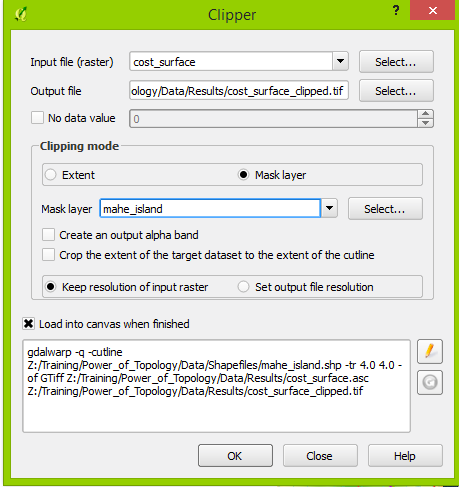
\includegraphics[width=8cm]{Images/clip_cost_surface.png}
	\caption{Clipping the cost surface}\label{fig:clip_cost_surface}
\end{figure}

After the clipping remove the original \textit{cost\_surface} layer from the table of contents. To clip the \textit{isochrones} use the \textit{Clip} tool from the \textit{Vector:Geoprocessing} menu (Figure \ref{fig:clip_isochrones}).

\begin{figure}[htb]
	\centering
	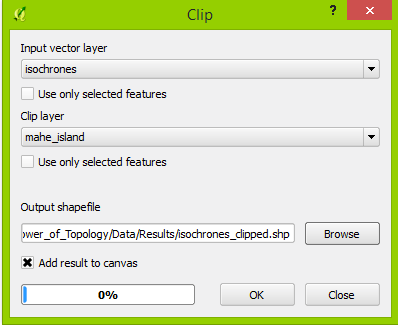
\includegraphics[width=8cm]{Images/clip_isochrones.png}
	\caption{Clipping the isochrones}\label{fig:clip_isochrones}
\end{figure}

Go to the style settings of the \textit{cost\_surface\_clipped} layer and apply the settings shown in Figure \ref{fig:cost_surface_style}. After clipping remove the original \textit{isochrones} layer from the table of contents.

\begin{figure}[htb]
	\centering
	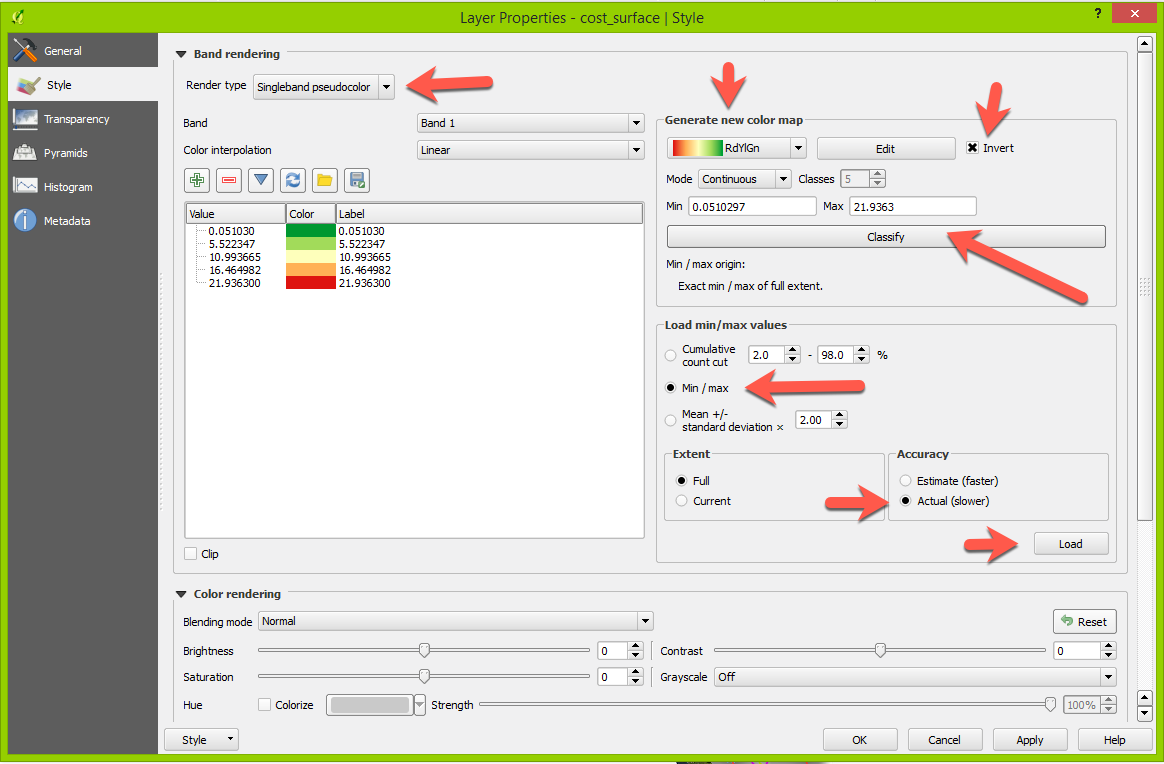
\includegraphics[width=12cm]{Images/cost_surface_style.png}
	\caption{Styling the cost surface}\label{fig:cost_surface_style}
\end{figure}

Finally label the \textit{isochrones\_clipped} layer with the values from the \textit{TIME} field/column. The final result map might look like Figure \ref{fig:final_map}.

\begin{figure}[htb]
	\centering
	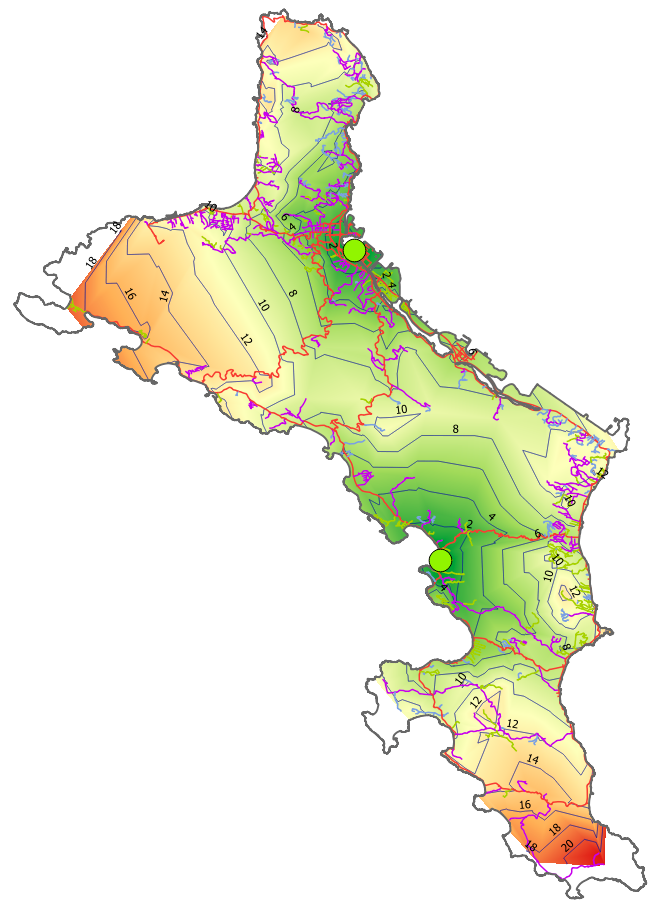
\includegraphics[width=14cm]{Images/final_map.png}
	\caption{Final map with isochrones, roads, fire stations and cost surface}\label{fig:final_map}
\end{figure}

\end{document}
